\begin{figure}
	% define source coordinates
	\begin{itemize}
		\item Anode \tikz[na] \coordinate (s-anode);
            \item Cathode \tikz[na] \coordinate (s-cathode);
            \item Saline bridge \tikz[na] \coordinate (s-bridge);
        \end{itemize}
        
        % Use a background grid to make it easier to find coordinates
        % When the coordinates have been found, remove the 
        % 'show background grid' option. 
        \tikzstyle{background grid}=[draw, black!50,step=.5cm]
        \begin{tikzpicture}[show background grid]
            % Put the graphic inside a node. This makes it easy to place the
            % graphic and to draw on top of it. 
            % The above right option is used to place the lower left corner
            % of the image at the (0,0) coordinate. 
            \node [inner sep=0pt,above right] 
			{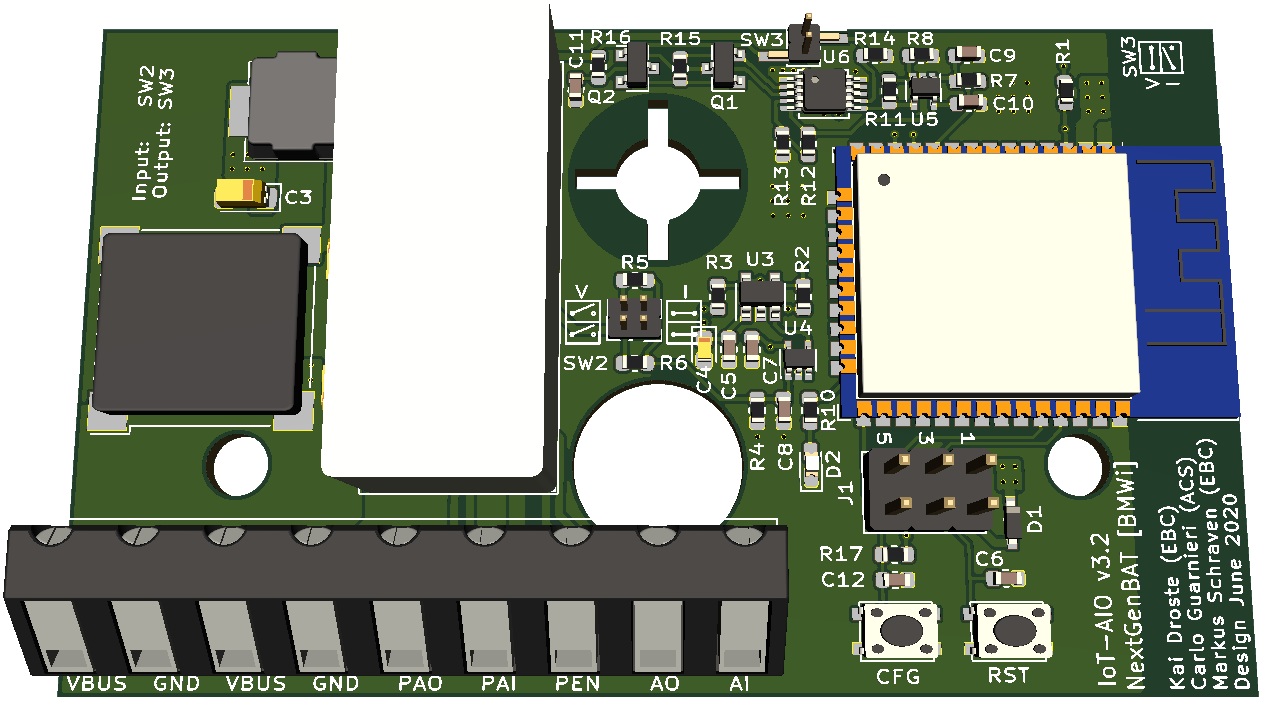
\includegraphics[width=\textwidth, opacity=.5]{Figures/analog.png}};
            % show origin
			\fill (0,0) circle (2pt);
			\draw[red, thick](3,0.25) circle (0.4);
            % define destination coordinates
            \path (0.7,2) coordinate (cathode)
			(3,0.25) coordinate (bridge)
			(2.75,2.5) coordinate (anode);
        \end{tikzpicture}
		
		
		% define overlays
		% Note the use of the overlay option. This is required when 
		% you want to access nodes in different pictures.
		\begin{tikzpicture}[overlay]
			\path[->,red,thick] (s-anode) edge [bend left] (anode);
			\path[->,blue,thick] (s-cathode) edge [bend left] (cathode);
			\path[->,red,thick] (s-bridge) edge [out=0, in=-90] (bridge);
		\end{tikzpicture}
	\end{figure}